\subsubsection{Non-Autonomous Iteration}
\index{Comerford, Mark}

\paragraph{Research Team}
Mark Comerford (Research Instructor)

\medskip

My research has been focused on investigating the properties of Julia sets
arising from arbitrary compositions of polynomials in $\C$. This generalizes
the standard situation of polynomial iteration in complex dynamics and as in
the standard case, one obtains a Fatou set, a Julia set and a filled Julia set.
The natural thing to do is then to ask which results from the existing theory
carry over as generalizations and to find counterexamples for those which do
not. What one tends to find is that the deeper results of complex dynamics such
as  Sullivan's non-wandering theorem and the classification of periodic Fatou
components do not carry over. However if one imposes some extra restrictions on
the dynamics of the sequences one considers, such as hyperbolicity or
semi-hyperbolicity, then much of the well-known results on hyperbolic and
semi-hyperbolic behaviour do generalize, although the old proofs no longer work
and new methods need to be developed.  

\paragraph{Highlights}

In 2006 I have been concerned largely with hyperbolic systems where one has
uniformly expanding dynamics on the Julia set. I have shown how a well-known
classical result which gives equivalent conditions to hyperbolicity can be
generalized. The proof required the development of new methods as those for the
classical proof were no longer available.  Building on this, I went on to show
how the Julia set moves smoothly and indeed holomorphically in the appropriate
sense in the neighbourhood of  a sequence where the associated dynamics is
hyperbolic. This again generalizes classical results but leads to some
unexpected and interesting conclusions concerning the parameter space. This
work is part of an over-reaching program of understanding parameter spaces for
non-autonomous iteration which  is analagous to the study of the Mandelbrot and
multibrot sets in standard polynomial iteration. 

\begin{figure}[ht]
  \begin{center}
    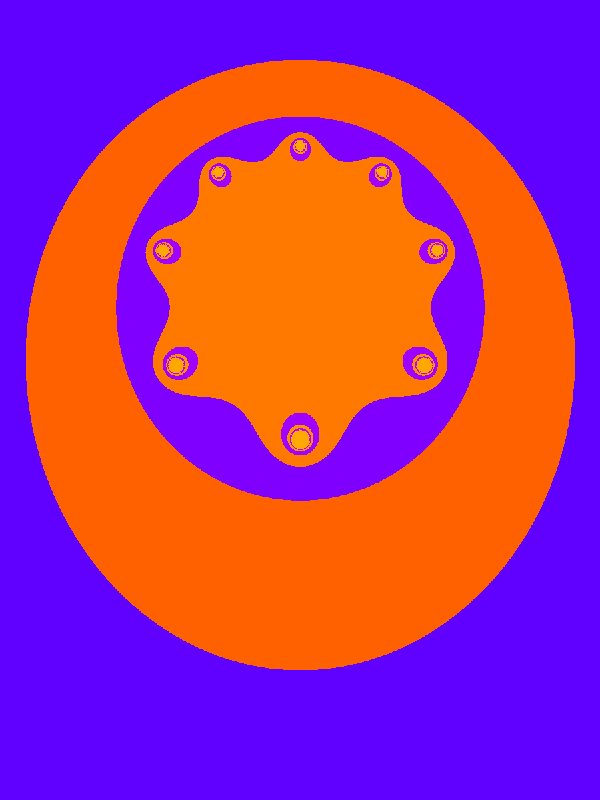
\includegraphics[width=\hsize]{Comerford/Figure23.png}
    \mycaption{A detail of a hyperbolic non-autonomous Julia set whose basin at infinity is not a John domain}\label{fig:profComerford}
   \end{center}
\end{figure}


Another part of this program is  a paper which will be the first stage towards
applying the work of Douady, Hubbbard and others on polynomial-like mappings
and renormalization. I started this paper some time ago while at Jacobs
University Bremen and am currently working towards a finished version to be
submitted for publication. 

Finally, while at Jacobs University and continuing here at the University of
Rhode Island, I have been working on trying to understand the geometry of the
Fatou set in the hyperbolic and semi-hyperbolic cases. This follows on from the
highly successful work of Carleson, Jones and Yoccoz who showed that in the
standard case of polynomial iteration, the dynamics on the Julia set is
semi-hyperbolic if and only if all the Fatou components are John domains. The
non-autonomous situation is more complicated, however, and one of the results
included in my paper on holomorphic motions which was written while at Jacobs
University gives an example of a sequence of polynomials with hyperbolic (and
hence semi-hyperbolic) dynamics where one has a Fatou component which is not a
John domain. The aim is to find an a priori weaker geometric condition which
describes the geometry of these domains but which is nevertheless still strong
enough to force semi-hyperbolic behaviour. However, much work still remains to
be done in this area. 


\nocite{Comerford1}
%\nocite{Comerford2}
%\nocite{Comerford3}
